\chapter{Bausteinsicht}

\section{Ebene 1}

Der Machtpunktezähler besteht aus vier Subsystemen. Die gestrichelten Pfeile stellen Abhängigkeiten der Subsysteme untereinander dar (x -> y für x ist abhängig von y). Die Kästchen im Äußeren Rand bilden die Kommunikationspunkte mit anderen Systemen bzw. Nutzern.

\begin{figure}[h]
\begin{center}
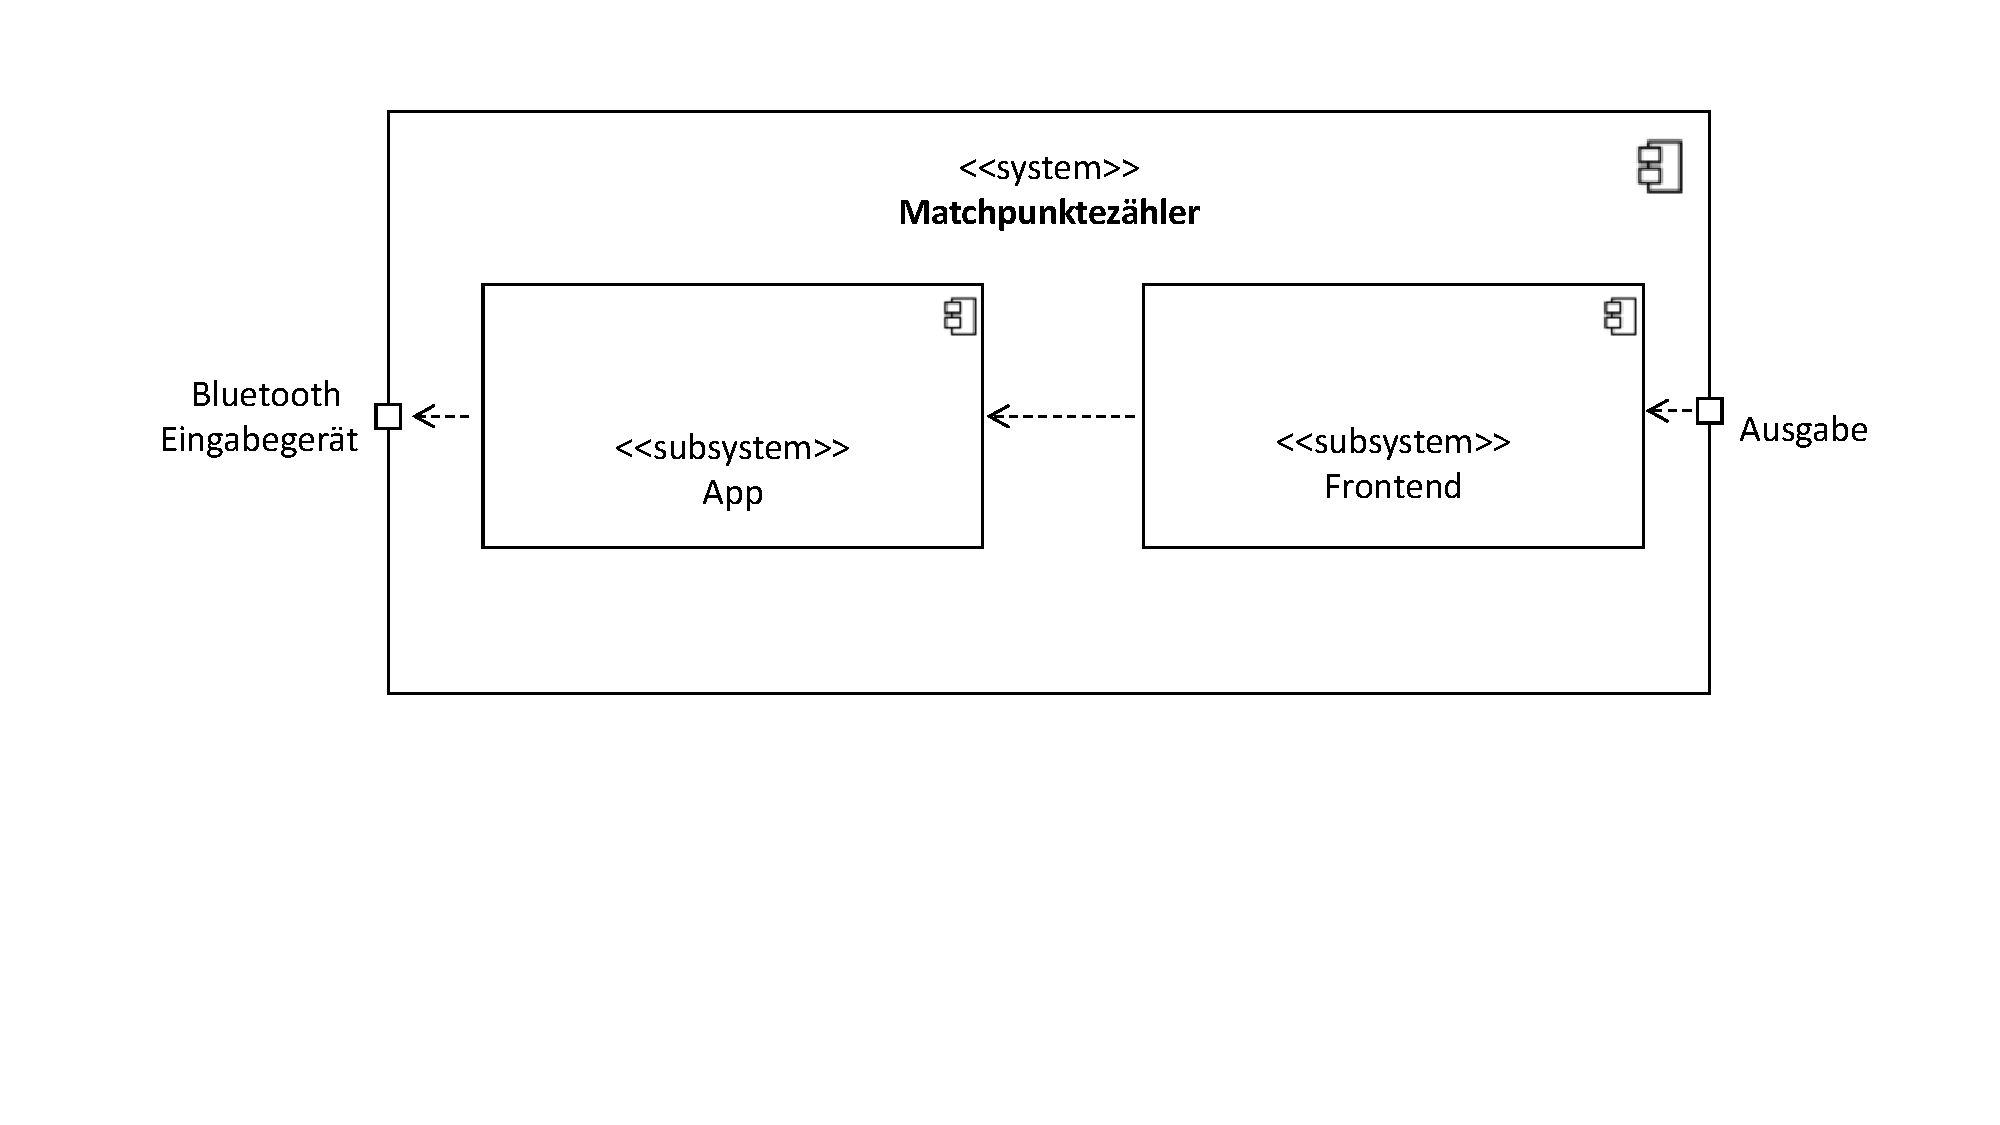
\includegraphics[scale=0.5]{Grafiken/Baustein_1.pdf}
\caption{Bausteinansicht Ebene 1}
\end{center}
\end{figure}

\begin{center}
\begin{tabular}[h]{|l|l|}
\cline{1-2}
\textbf{Subsystem} & \textbf{Kurzbeschreibung}\\
\cline{1-2}
App & Realisiert die Kommunikation, Verarbeitung der Eingaben\\&und Umsetzung der Spielregeln.\\ 
\cline{1-2}
Frontend & Stellt anhand der vom Backend gegebenen Daten den Zustand der App grafisch aus.\\
\cline{1-2} 
\end{tabular}
\end{center}

\section{App}
\subsection*{Zweck/Verantwortlichkeit}
Das Subsystem repräsentiert die Kommunikation und  die Signalverarbeitung. Eingabe von externen Geräten werden interpretiert und für die Ausgabe über das Subsystem Frontend vorbereitet.
\subsection*{Schnittstellen}
\subsection*{Ablageort / Datei}
/MatchPunktezaehler/src/flask\_sse\_project/app/
\subsection*{Offene Punkte}
Offene Punkte werden in den einzelnen Modulen dieses Subsystems in Ebene 2 \ref{sec:App} beschrieben.

\section{Frontend}
\subsection*{Zweck/Verantwortlichkeit}
Das Subsystem ist für die graphische Ausgabe der in dem Subsystem App ermittelten Daten verantwortlich. Diese werden für den Endnutzer passend aufbereitet.
\subsection*{Schnittstellen}
Das Frontend beinhaltet so gut wie keine Eigene Logik und baut auf den Daten des Subsystems App auf.
\subsection*{Ablageort / Datei}
/MatchPunktezaehler/src/flask\_sse\_project/frontend/
\subsection*{Offene Punkte}
\begin{itemize}
	\item Implementierung mehrerer Spieletypen.
\end{itemize}

\newpage

\section{Ebene 2: App}
\label{sec:App}
Das Subsystem App zerfällt in folgende Einzelmodule. Diese übernehmen die Kommunikation zwischen den Modulen/Subsystemen und Interpretation/Verarbeitung der Eingaben.

\begin{figure}[H]
\begin{center}
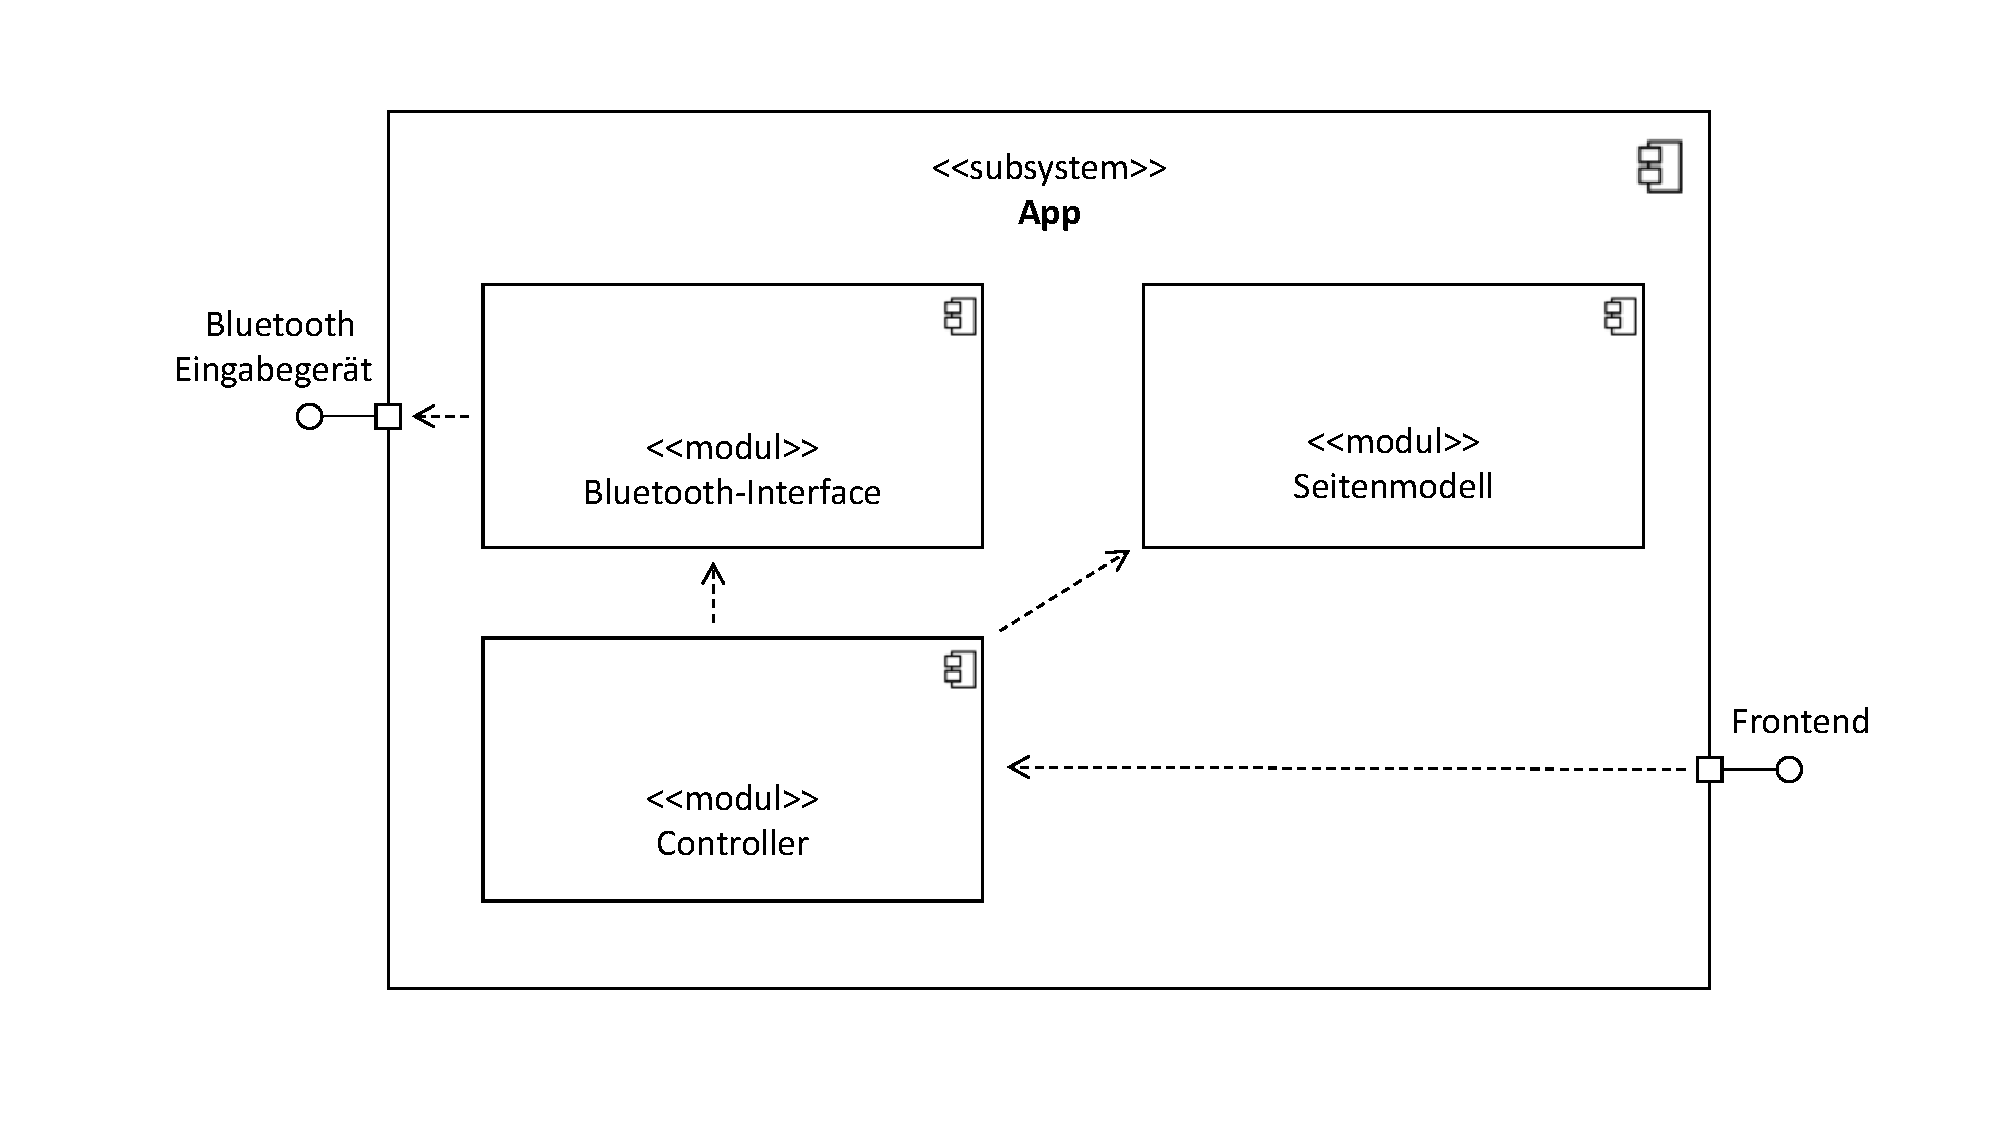
\includegraphics[scale=0.5]{Grafiken/Baustein_2.pdf}
\caption{Bausteinansicht Ebene 2: App}
\end{center}
\end{figure}

\section{Controller}
\subsection*{Zweck/Verantwortlichkeit}
Das Subsystem realisiert die Kommunikation zwischen den Subsystemen (z.B. mit dem Frontend). Bei einer Eingabe über das Subsystem Bluetooth-Interface werden über den Controller mit Hilfe der Spielregeln die Daten für die Ausgabe über das Frontend ermittelt.
\subsection*{Schnittstellen}
Das Modul repräsentiert seine Funktionalität über folgende Methoden.
\begin{center}
\begin{tabular}[h]{|l|l|}
\cline{1-2}
\textbf{Methode} & \textbf{Kurzbeschreibung}\\
\cline{1-2}
readBluetooth & Liest asynchron die Eingabe des Bluetooth-Eingabegerätes ein.\\ 
\cline{1-2}
setupBluetoothThread & Erstellt einen Thread für die Bluetooth-Kommunikation.\\
\cline{1-2}
startGame & Erstellt ein neues Spiel.\\
\cline{1-2}
UpdateSite & Gibt neue Parameter an das Frontend.\\
\cline{1-2} 
\end{tabular}
\end{center}
\subsection*{Ablageort / Datei}
/MatchPunktezaehler/src/flask\_sse\_project/app/flaskr/controller.py
\subsection*{Offene Punkte}
\begin{itemize}
	\item Implementierung einer Datenbankschnittstelle für Langzeitstatistiken.
\end{itemize}

\section{Seitenmodell}
\subsection*{Zweck/Verantwortlichkeit}
Das Subsystem bietet die Grundlage zur Funktionsweise des Systems. Es werden die Eingaben gemäß des Spielertypen interpretiert und in eine Ausgabe an das Frontend umgewandelt.
\subsection*{Schnittstellen}
Das Modul repräsentiert seine Funktionalität über folgende Methoden.
\begin{center}
\begin{tabular}[h]{|l|l|}
\cline{1-2}
\textbf{Methode} & \textbf{Kurzbeschreibung}\\
\cline{1-2}
CounterUp & Erhöht Spielstand für ein Team.\\ 
\cline{1-2}
Undo & Stellt den zuvor bestandenen Spielstand wieder her.\\
\cline{1-2}
Redo & Macht ein Undo wieder Rückgängig .\\
\cline{1-2}
UpdatePlayerPosition & Gibt die aktuellen Positionen der Spieler zurück.\\
\cline{1-2} 
UpdateServePosition & Gibt die Momentane Aufschlagposition zurück.\\
\cline{1-2}
\end{tabular}
\end{center}
\subsection*{Ablageort / Datei}
/MatchPunktezaehler/src/flask\_sse\_project/app/flaskr/model/
\subsection*{Offene Punkte}
\begin{itemize}
	\item Implementierung mehrerer Spieltypen.
\end{itemize}

\section{Bluetooth-Interface}
\subsection*{Zweck/Verantwortlichkeit}
Das Subsystem ist für das Verbinden und die Kommunikation mit einem Bluetooth-Eingabegerät verantwortlich. Somit wird am Anfang die Verbindung mit dem Eingabegerät hergestellt und anschließend bei einer Betätigung die Eingabe eingelesen und vor interpretiert.
\subsection*{Schnittstellen}
Das Modul repräsentiert seine Funktionalität über folgende Methoden.
\begin{center}
\begin{tabular}[h]{|l|l|}
\cline{1-2}
\textbf{Methode} & \textbf{Kurzbeschreibung}\\
\cline{1-2}
readBluetooth & Liest asynchron die Eingabe des Bluetooth-Interfaces ein.\\ 
\cline{1-2}
findDevice & Sucht ein bereits verbundenes Eingabegerät merkt es sich.\\
\cline{1-2}
deviceCount & Gibt die Anzahl an verbundenen Geräten wieder (max 1).\\
\cline{1-2}
UpdatePlayerPosition & Gibt die aktuellen Positionen der Spieler zurück.\\
\cline{1-2} 
UpdateServePosition & Gibt die Momentane Aufschlagposition zurück.\\
\cline{1-2}\cline{1-2} 
\end{tabular}
\end{center}
\subsection*{Ablageort / Datei}
/MatchPunktezaehler/src/flask\_sse\_project/app/flaskr/bluetooth\_controller.py
\subsection*{Offene Punkte}
\begin{itemize}
	\item Verbinden mit mehreren Bluetooth-Eingabegeräten ermöglichen.
	\item Zuverlässigere Methode zum Koppeln neuer Geräte implementieren.
\end{itemize}
